\documentclass[10pt,a4paper]{article}
\usepackage[margin=17mm,headheight=12pt,headsep=5mm,footskip=8mm]{geometry}
\usepackage{lmodern,amsmath,graphicx,booktabs,tabularx,array,xcolor,caption,fancyhdr,xurl}
\usepackage[colorlinks=true,linkcolor=teal,urlcolor=teal]{hyperref}
\definecolor{navy}{HTML}{182D45}
\definecolor{teal}{HTML}{147D83}
\definecolor{muted}{HTML}{526376}
\hypersetup{pdftitle={RaspFormer: results summary},pdfauthor={RaspFormer project},pdfsubject={Concise research results on representation geometry and computation}}
\setlength{\parindent}{0pt}
\setlength{\parskip}{4pt}
\setlength{\tabcolsep}{5pt}
\renewcommand{\arraystretch}{1.15}
\renewcommand{\tabularxcolumn}[1]{>{\raggedright\arraybackslash}p{#1}}
\setlength{\emergencystretch}{1.5em}
\captionsetup{font=footnotesize,labelfont=bf,labelsep=period,skip=3pt,justification=raggedright,singlelinecheck=false,hypcap=false}
\pagestyle{fancy}
\fancyhf{}
\fancyhead[L]{\sffamily\footnotesize\color{muted}RASPFORMER / RESULTS}
\fancyhead[R]{\sffamily\footnotesize\color{muted}18 October 2026}
\fancyfoot[L]{\footnotesize\color{muted}Reference experiments recorded 15 October 2026.}
\fancyfoot[R]{\footnotesize\thepage}
\renewcommand{\headrulewidth}{.3pt}
\newcommand{\heading}[1]{\par\vspace{2pt}{\sffamily\bfseries\color{navy}#1}\par}

\begin{document}
{\sffamily\large\bfseries\color{navy}Results}\par
\textbf{Principal finding.} Participation ratio (PR) and centered kernel alignment (CKA) detect some first-write timing. High timing scores can coexist with poor task accuracy, limiting claims of computation recovery.

\heading{1. Blind timing detection succeeds on average}
On six held-out programs, PR and CKA achieve macro F1 of \textbf{0.853} and \textbf{0.850}, versus 0.745 for always writing. A simpler residual-change detector scores \textbf{0.876}. Activation-only predictions are frozen before schedule scoring; P11 CKA falls below its own baseline.

\heading{2. Compression exposes a gap between geometry and behavior}
Across twelve tasks, target half-width uncentered SVD gives \textbf{61.62\%} token accuracy, random projection 37.01\%, and full rank 100\%. On the held-out six, random compression reaches \textbf{0.879 CKA schedule F1} with \textbf{37.62\% task accuracy} (Figure~1). The schedule remains an intended reference. Attention/MLP hidden dimensions stay fixed.

\par\begingroup\centering
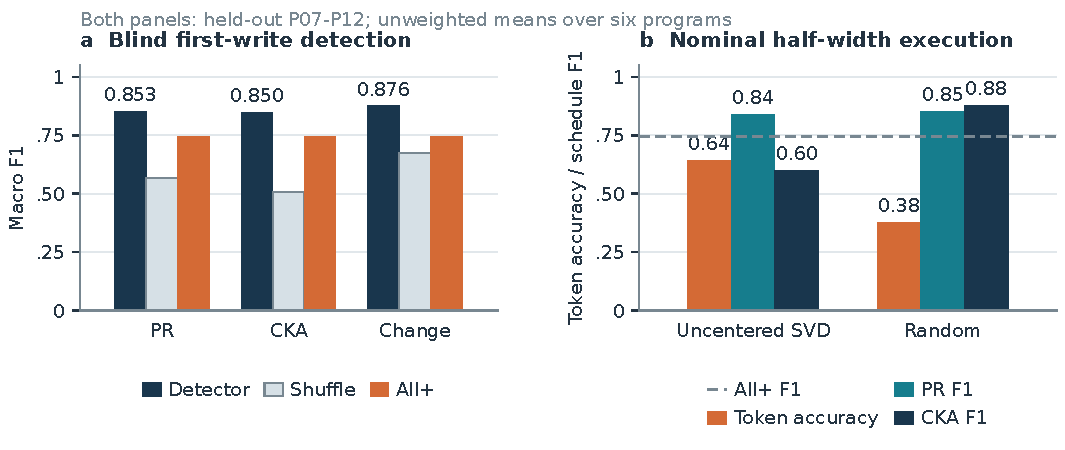
\includegraphics[width=.90\linewidth]{figures/recovery-compression.pdf}
\captionof{figure}{Unweighted means over six held-out programs, P07 to P12. Left: blind detection and baselines. Right: half-width execution. The original intended schedule is not established causal ground truth for the compressed models.}
\par\endgroup

\heading{3. PCA patches provide limited causal evidence}
Rank-three principal component analysis (PCA) patches match symbolic counterfactuals on \textbf{113/192 pairs (58.85\%)}, versus 42.19\% for equal-rank random directions and 47.92\% for self patches. Conditions share 192 pairs across twelve tasks. PCA patches alter outputs in 26 pairs; variable mapping is supervised. All 60 undefined condition rows remain failures. Comparisons are descriptive.

\heading{4. Control experiments}
\begingroup\small
\begin{tabularx}{\linewidth}{@{}>{\raggedright\arraybackslash}p{.17\linewidth}X@{}}
\toprule
\textbf{Control} & \textbf{Result and interpretation}\\
\midrule
Numerical policy & Total sample-variance floor $10^{-12}$ reduces CKA availability mismatches from 14 to 2 across 54 transitions. Helper-state timing explains the remaining cases.\\
Sorting errors & Each lane fails 64/512 probes; sets are disjoint. Doubling QK-logit scale lowers maximum error from $8.52\times10^{-4}$ to $7.15\times10^{-7}$; decoded accuracy stays 100\%.\\
Rotation & All 36 executed orthogonal transforms preserve 100\% output agreement. Maximum posthoc PR/CKA error is $1.42\times10^{-13}$; original-lane checks change.\\
Structural design & Nine crossed depth/branch-count variants yield rank-two realized depth/count, removing exact collinearity. No general complexity law is established.\\
\bottomrule
\end{tabularx}
\endgroup

\heading{5. Learned-model transfer}
Across 36 trained transformers, per-task mean test accuracy is \textbf{95.41\% to 100\%}; palindrome's majority baseline is 93.94\%. Final learned/compiled CKA spans 0.152 to 0.802. Learned final PR is lower for every task; internal circuits remain unknown.

\heading{Conclusion}
The evidence supports partial timing recovery and modest geometry-directed intervention effects. The original fidelity comparison uses compiler-known encodings; PR depends on encoding and scale. Complete algorithm discovery, erasure, lifetimes, and semantic superposition recovery remain open. No direct InterpBench benchmark was run.

\begingroup\footnotesize\raggedright
\textbf{Setup.} Length six; vocabulary eight. Compiled calibration/test sets contain 96/96 disjoint sequences. Learned train/validation/test splits contain 2,029/677/677 sequences, with three seeds. No experiments were rerun.
\href{https://github.com/raghulchandramouli/RaspFormer/tree/e06479ce09f10695aa5280162f80d880c060eaf5}{Canonical evidence, e06479c}.
\endgroup
\end{document}
